\section{Auswertung}
\label{sec:Auswertung}
In diesem Kapitel sollen die aufgenommenen Messwerte Ausgewertet werden.
\subsection{Lineare bestimmung von $RC$}
\label{sec:auswertungeins}
Um einen Wert für die Konstante $RC$ zu ermitteln, werden zunächst vom Oszilloskop einige Wertepaare
für die Zeit $t$ und die zugehörige Spannung $U$ aufgenommen, diese werden ins Verhältnis
zu $U_0=\SI[]{12}[]{V}$ gesetzt und in \autoref{fig:aufladevorgang} halblogarithmisch dargestellt.
An die Messpunkte wird dann mit der numpy.polyfit Funktion ein Polynom ersten grades angepasst, aus
dessen Steigung dann auf den Wert für $RC$ geschlossen werden kann. Das Polynom hat die Form:
\begin{center}
    $-ln(\frac{U}{U_0})=\frac{t}{RC}+b$\\
\end{center}
mit den durch python berechnetenParametern:
\begin{center}
    $RC=\SI[]{(5.6\pm0.7)\times 10^{-3}}[]{s}$\\
    $b=0.17341742 \pm 0.05212717$
\end{center}
\begin{figure}
    \centering
    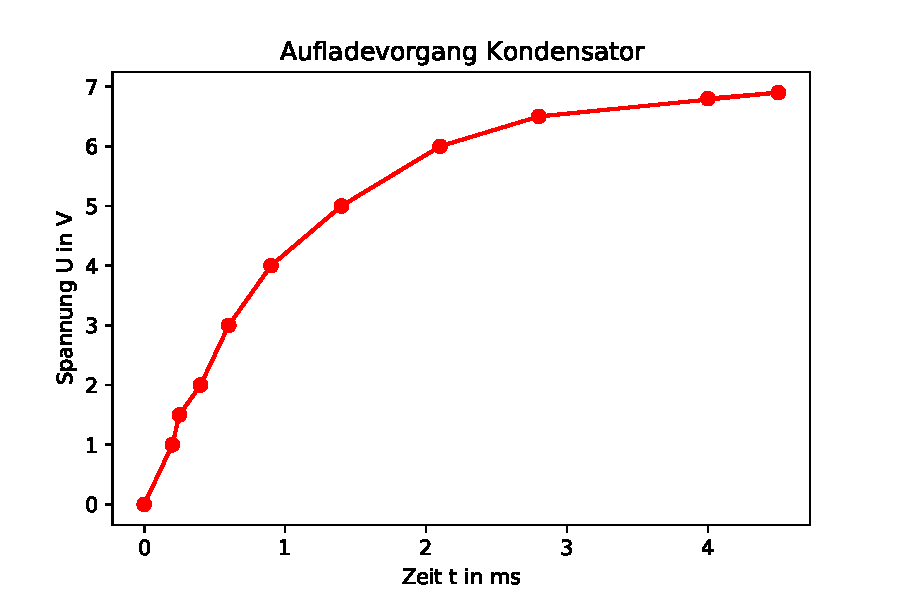
\includegraphics{aufladevorgang.pdf}
    \caption{Aufladevorgang eines Kondensators}
    \label{fig:aufladevorgang}
  \end{figure}

\subsection{Bestimmung von RC anhand der Frequenz}
\label{sec:auswertungzwei}
Als nächstes werden Wertepaare aus Spitze-Spitze-Spannung $U_{SS}$ und Frequenz $f$ aufgenommen und auf gleiche Weise 
wie in \autoref{sec:auswertungeins} in \autoref{fig:kondensatorspannung} dargestellt. An diese 
Messwerte wurde eine Funktion der Form:
\begin{center}
    $\frac{U_{SS}}{U_0}=\frac{1}{\sqrt{4\pi^2 f^2 R^2C^2}}$\\
\end{center}
mithilfe der scipy.curve_fit Funktion angepasst. Dabei ergab sich der Wert:
\begin{center}
    $RC=\SI[]{(1.5046 \pm 0.0986)\times 10^{-3}}[]{s}$\\
\end{center}
\begin{figure}
    \centering
    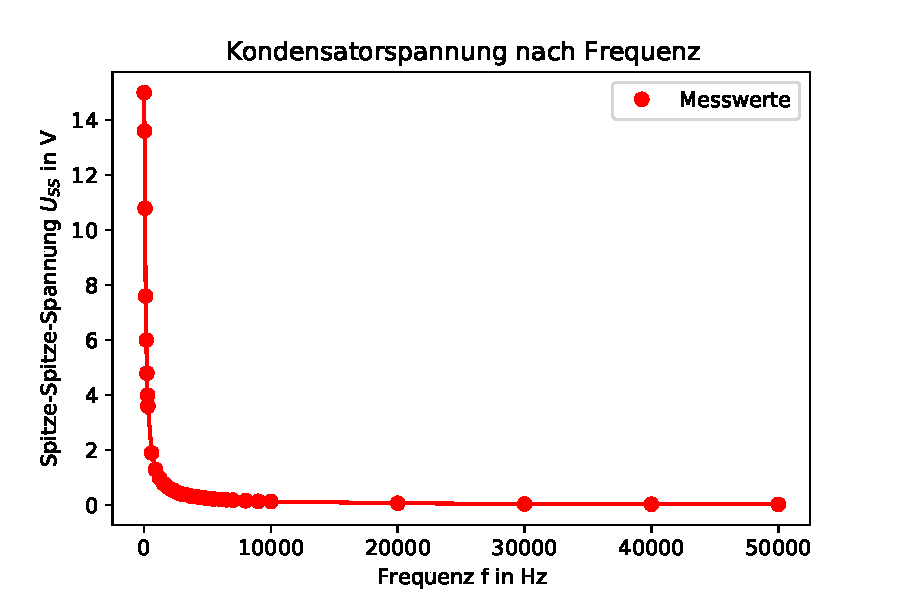
\includegraphics{Kondensatorspannung.pdf}
    \caption{kondensatorspannung in Abhängigkeit der Frequenz}
    \label{fig:kondensatorspannung}
  \end{figure}

\subsection{Bestimmmung von RC  anhand der Phasenverschiebung}
\label{sec:auswertungdrei}
Im folgenden wird die Phasenverschiebung in Abhängigkeit zur Frequenz gemessen. Dazu wird die Verschiebung
zwischen den beiden Maxima vom Oszilloskop abgelesen und mittels:
\begin{center}
    $b=\frac{c}{f}$\\
    $\phi=2\pi \frac{a}{b}$\\
\end{center}
in Winkel umgerechnet. Anschließend wird eine Kurve der Form:
\begin{center}
    $\phi=a *arctan(f*RC)$
\end{center}
angepasst. Dies führt zu einem Wert von:
\begin{center}
    $RC=\SI[]{(14.37 \pm 5.81)\times10^{-3}}[]{s}$
\end{center}
Der zugehörige Plot ist in \autoref{fig:verschiebung} zu sehen.
\begin{figure}
    \centering
    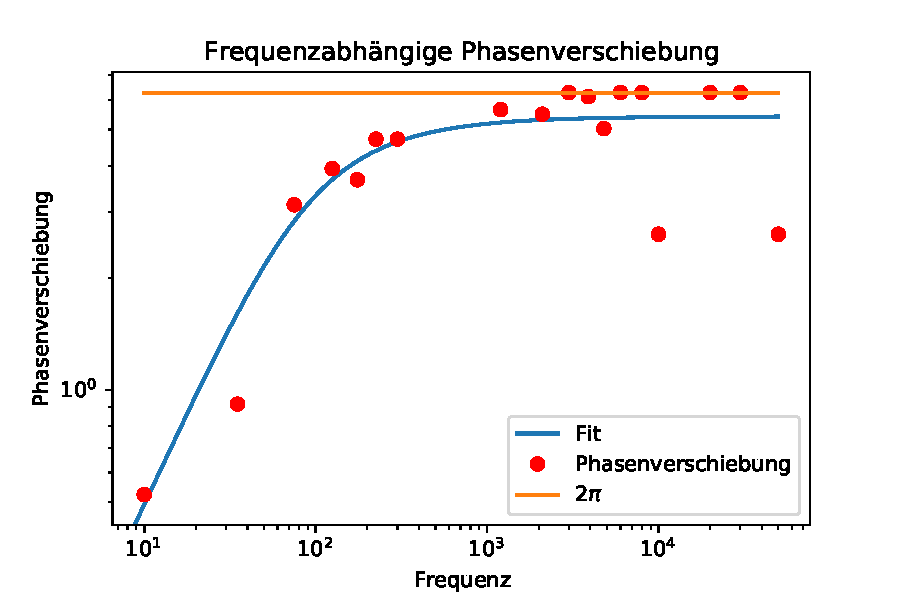
\includegraphics{verschiebung.pdf}
    \caption{Phasenverschiebung}
    \label{fig:verschiebung}
  \end{figure}
In \autoref{fig:polarplot} wird die Spannung $U_{SS}$ gegen die Phasenverschiebung $\phi$ aufgetragen.
  \begin{figure}
    \centering
    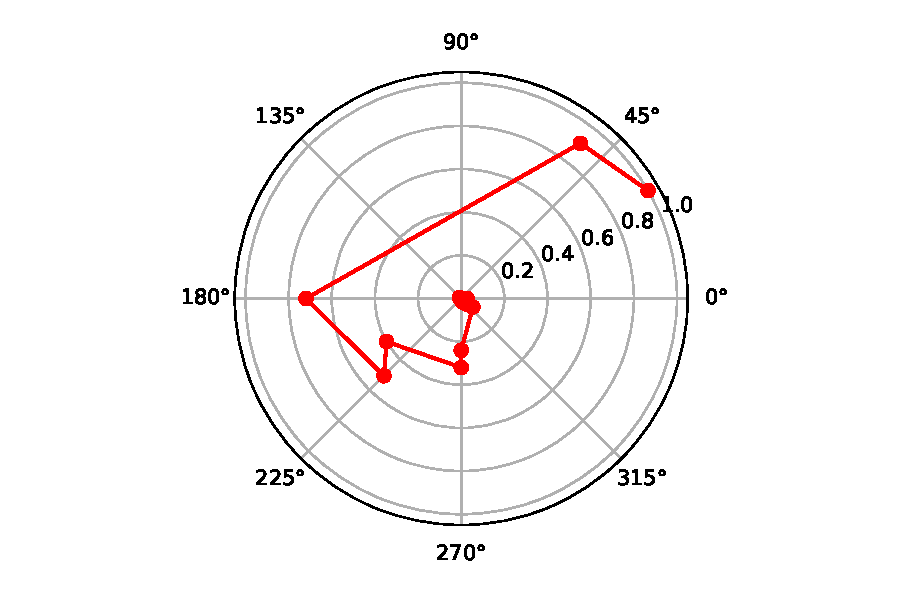
\includegraphics{polar.pdf}
    \caption{Phasenverschiebung pro Spannung}
    \label{fig:polarplot}
  \end{figure}